% Options for packages loaded elsewhere
\PassOptionsToPackage{unicode}{hyperref}
\PassOptionsToPackage{hyphens}{url}
\PassOptionsToPackage{dvipsnames,svgnames,x11names}{xcolor}
%
\documentclass[
  letterpaper,
  DIV=11,
  numbers=noendperiod]{scrartcl}

\usepackage{amsmath,amssymb}
\usepackage{lmodern}
\usepackage{iftex}
\ifPDFTeX
  \usepackage[T1]{fontenc}
  \usepackage[utf8]{inputenc}
  \usepackage{textcomp} % provide euro and other symbols
\else % if luatex or xetex
  \usepackage{unicode-math}
  \defaultfontfeatures{Scale=MatchLowercase}
  \defaultfontfeatures[\rmfamily]{Ligatures=TeX,Scale=1}
\fi
% Use upquote if available, for straight quotes in verbatim environments
\IfFileExists{upquote.sty}{\usepackage{upquote}}{}
\IfFileExists{microtype.sty}{% use microtype if available
  \usepackage[]{microtype}
  \UseMicrotypeSet[protrusion]{basicmath} % disable protrusion for tt fonts
}{}
\makeatletter
\@ifundefined{KOMAClassName}{% if non-KOMA class
  \IfFileExists{parskip.sty}{%
    \usepackage{parskip}
  }{% else
    \setlength{\parindent}{0pt}
    \setlength{\parskip}{6pt plus 2pt minus 1pt}}
}{% if KOMA class
  \KOMAoptions{parskip=half}}
\makeatother
\usepackage{xcolor}
\setlength{\emergencystretch}{3em} % prevent overfull lines
\setcounter{secnumdepth}{-\maxdimen} % remove section numbering
% Make \paragraph and \subparagraph free-standing
\ifx\paragraph\undefined\else
  \let\oldparagraph\paragraph
  \renewcommand{\paragraph}[1]{\oldparagraph{#1}\mbox{}}
\fi
\ifx\subparagraph\undefined\else
  \let\oldsubparagraph\subparagraph
  \renewcommand{\subparagraph}[1]{\oldsubparagraph{#1}\mbox{}}
\fi


\providecommand{\tightlist}{%
  \setlength{\itemsep}{0pt}\setlength{\parskip}{0pt}}\usepackage{longtable,booktabs,array}
\usepackage{calc} % for calculating minipage widths
% Correct order of tables after \paragraph or \subparagraph
\usepackage{etoolbox}
\makeatletter
\patchcmd\longtable{\par}{\if@noskipsec\mbox{}\fi\par}{}{}
\makeatother
% Allow footnotes in longtable head/foot
\IfFileExists{footnotehyper.sty}{\usepackage{footnotehyper}}{\usepackage{footnote}}
\makesavenoteenv{longtable}
\usepackage{graphicx}
\makeatletter
\def\maxwidth{\ifdim\Gin@nat@width>\linewidth\linewidth\else\Gin@nat@width\fi}
\def\maxheight{\ifdim\Gin@nat@height>\textheight\textheight\else\Gin@nat@height\fi}
\makeatother
% Scale images if necessary, so that they will not overflow the page
% margins by default, and it is still possible to overwrite the defaults
% using explicit options in \includegraphics[width, height, ...]{}
\setkeys{Gin}{width=\maxwidth,height=\maxheight,keepaspectratio}
% Set default figure placement to htbp
\makeatletter
\def\fps@figure{htbp}
\makeatother

\KOMAoption{captions}{tableheading}
\makeatletter
\makeatother
\makeatletter
\makeatother
\makeatletter
\@ifpackageloaded{caption}{}{\usepackage{caption}}
\AtBeginDocument{%
\ifdefined\contentsname
  \renewcommand*\contentsname{Table of contents}
\else
  \newcommand\contentsname{Table of contents}
\fi
\ifdefined\listfigurename
  \renewcommand*\listfigurename{List of Figures}
\else
  \newcommand\listfigurename{List of Figures}
\fi
\ifdefined\listtablename
  \renewcommand*\listtablename{List of Tables}
\else
  \newcommand\listtablename{List of Tables}
\fi
\ifdefined\figurename
  \renewcommand*\figurename{Figure}
\else
  \newcommand\figurename{Figure}
\fi
\ifdefined\tablename
  \renewcommand*\tablename{Table}
\else
  \newcommand\tablename{Table}
\fi
}
\@ifpackageloaded{float}{}{\usepackage{float}}
\floatstyle{ruled}
\@ifundefined{c@chapter}{\newfloat{codelisting}{h}{lop}}{\newfloat{codelisting}{h}{lop}[chapter]}
\floatname{codelisting}{Listing}
\newcommand*\listoflistings{\listof{codelisting}{List of Listings}}
\makeatother
\makeatletter
\@ifpackageloaded{caption}{}{\usepackage{caption}}
\@ifpackageloaded{subcaption}{}{\usepackage{subcaption}}
\makeatother
\makeatletter
\@ifpackageloaded{tcolorbox}{}{\usepackage[many]{tcolorbox}}
\makeatother
\makeatletter
\@ifundefined{shadecolor}{\definecolor{shadecolor}{rgb}{.97, .97, .97}}
\makeatother
\makeatletter
\makeatother
\ifLuaTeX
  \usepackage{selnolig}  % disable illegal ligatures
\fi
\IfFileExists{bookmark.sty}{\usepackage{bookmark}}{\usepackage{hyperref}}
\IfFileExists{xurl.sty}{\usepackage{xurl}}{} % add URL line breaks if available
\urlstyle{same} % disable monospaced font for URLs
\hypersetup{
  pdftitle={Big Bang Theory},
  colorlinks=true,
  linkcolor={blue},
  filecolor={Maroon},
  citecolor={Blue},
  urlcolor={Blue},
  pdfcreator={LaTeX via pandoc}}

\title{Big Bang Theory}
\author{}
\date{4/20/23}

\begin{document}
\maketitle
\ifdefined\Shaded\renewenvironment{Shaded}{\begin{tcolorbox}[borderline west={3pt}{0pt}{shadecolor}, breakable, sharp corners, boxrule=0pt, interior hidden, enhanced, frame hidden]}{\end{tcolorbox}}\fi

\listoffigures
\listoftables
\textsuperscript{\emph{This~report~will~summarize~and~analyze~the~Big~Bag~Theory's~viewership.}}

\hypertarget{brief-description}{%
\subsection{1. Brief Description}\label{brief-description}}

The Big Bang Theory is an American television sitcom created by Chuck
Lorre and Bill Prady, both of whom served as executive producers on the
series, along with Steven Molaro. The three of them also served as head
writers. It premiered on CBS on September 24, 2007, and concluded on May
16, 2019, having broadcast 279 episodes over 12 seasons.

\hypertarget{photo-of-the-show}{%
\subsection{2. Photo Of The Show}\label{photo-of-the-show}}

\begin{figure}

{\centering 
\includegraphics{The_Big_Bang_Theory.png}

}

\caption{Big Bang Theory}

\end{figure}

\hypertarget{a-summary-of-viewership}{%
\subsection{3. A Summary Of Viewership}\label{a-summary-of-viewership}}

\begin{longtable}[]{@{}lcr@{}}
\toprule()
Season & Epi. & U.S. Viewers(millions) \\
\midrule()
\endhead
1 & 17 & 8.31 \\
2 & 23 & 10.03 \\
3 & 23 & 14.22 \\
4 & 24 & 13.21 \\
5 & 24 & 15.82 \\
6 & 24 & 18.68 \\
7 & 24 & 19.96 \\
8 & 24 & 19.05 \\
9 & 24 & 20.36 \\
10 & 24 & 18.99 \\
11 & 24 & 18.63 \\
12 & 24 & 17.31 \\
\bottomrule()
\end{longtable}

Source:
\href{https://en.wikipedia.org/wiki/The_Big_Bang_Theory}{Wikipedia}

\hypertarget{a-graph-of-the-viewership-per-season}{%
\subsection{4 \& 5. A Graph Of The Viewership Per
Season}\label{a-graph-of-the-viewership-per-season}}

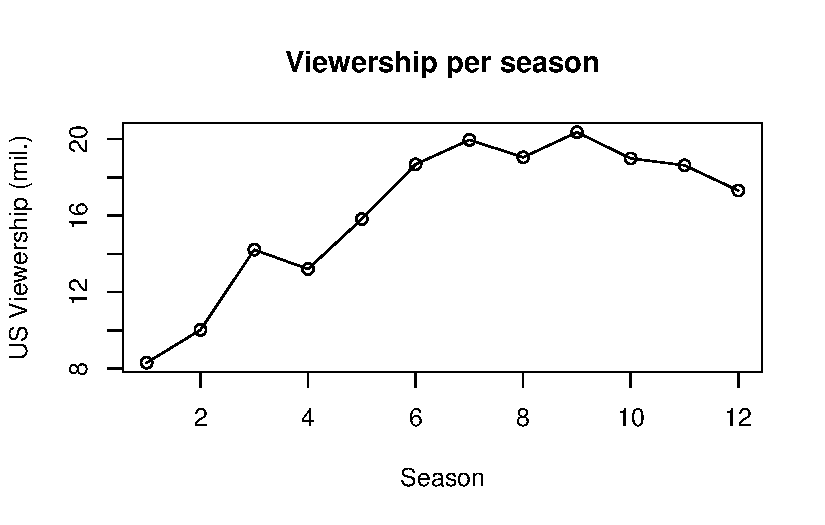
\includegraphics{Assignment2_files/figure-pdf/unnamed-chunk-1-1.pdf}

\hypertarget{viewership-analysis}{%
\subsection{6. Viewership Analysis}\label{viewership-analysis}}

\emph{Big Bang Theory} is the best sitcom of the recent decade.

In general, the viewership was on an upward trend. Viewership nearly
doubled, reaching \textbf{15.82 mil.} views by season 5. Before, peaking
at \textbf{20.36 mil.} views in season 9. Then, the viewership slightly
decreased, making up to \textbf{17.31 mil.} views at final season.



\end{document}
